\chapter{Опис додатку з використанням кросс-платформених рішень}
\label{ch2}


\section{Структура проекту в React Native}
\label{sec:rn_structure_app}

\begin{lstlisting}[style=light, language=Python,label={lst:rn_app_structure},caption=React Native App Layout]
├── App.js (1)
├── Readme.md
├── __tests__ (2)
│ └── App.js
├── android (3)
│ ├── app
│ ├── build
│ ├── build.gradle
│ ├── gradle
│ ├── gradle.properties
│ ├── gradlew
│ ├── gradlew.bat
│ ├── local.properties
│ └── settings.gradle
├── app.json (5)
├── babel.config.js (6)
├── index.js (7)
├── ios (4)
│ ├── BreedRN
│ ├── BreedRN.xcodeproj
│ ├── BreedRN.xcworkspace
│ ├── Podfile
│ ├── Podfile.lock
│ └── Pods
├── metro.config.js (8)
├── node_modules (11)
├── package-lock.json (10)
└── package.json (9)
\end{lstlisting}

\begin{enumerate}
    \item \textbf{App.js} сирцевий код нашого додатку
    \item \textbf{\_\_tests\_\_} сирцевий код тестів
    \item \textbf{android} сирцевий код платформеного коду Android
    \item \textbf{ios} сирцевий код платформеного коду iOS
    \item \textbf{app.json} конфігурує багато речей, від назви вашого додатка до піктограми до заставки, і навіть схеми глибоких зв’язків та ключів API для використання для деяких служб
    \item \textbf{babel.config.js} конфігурує Babel - це набір інструментів, який в основному використовується для перетворення коду ECMAScript 2015+ у зворотну сумісну версію JavaScript у поточних та старих браузерах або середовищах.
    \item \textbf{index.js} точка входу для React Native з цього файлу Javascript Engine вивантажує в пам'ять логіку додатку
    \item \textbf{metro.config.js} конфігурує Metro пакувальник JavaScript для платформ Android та iOS
    \item \textbf{package.json} конфігурує дерево залежностей або бібліотек, що використовує проект
    \item \textbf{package-lock.json} файл що описує повністю дерево залежностей, таким чином створює відтворюване середовище
    \item \textbf{node\_modules} репозиторій артефактів або сирцевого коду всіх Javascript пакетів, що використовує проект
\end{enumerate}


\section{Структура проекту в Flutter}
\label{sec:flutter_structure_app}

\begin{lstlisting}[style=light, language=Python,label={lst:flutter_project_layout},caption=Flutter Project Layout]
├── README.md
├── android (1)
│ ├── app
│ ├── build.gradle
│ ├── gradle
│ ├── gradle.properties
│ ├── gradlew
│ ├── gradlew.bat
│ ├── local.properties
│ └── settings.gradle
├── build (2)
├── ios (3)
│ ├── Flutter
│ ├── Podfile
│ ├── Runner
│ ├── Runner.xcodeproj
│ └── Runner.xcworkspace
├── lib (4)
│ ├── breed_list.dart
│ ├── data
│ ├── domain
│ ├── home.dart
│ ├── main.dart
│ └── presentation
├── pubspec.lock (5)
├── pubspec.yaml (6)
├── test (7)
│ ├── breed_database_test.dart
│ ├── breed_list_view_model_test.dart
│ ├── breed_list_view_model_test.mocks.dart
│ └── network_test.dart
└── web (8)
    ├── favicon.png
    ├── icons
    ├── index.html
    └── manifest.json
\end{lstlisting}

\begin{enumerate}
    \item \textbf{android} сирцевий код платформеного коду Android.
    \item \textbf{build} папка з тимчасовими файлами згенерованими Flutter CLI під час побудування проекту.
    \item \textbf{ios} сирцевий код платформеного коду iOS.
    \item \textbf{lib} сирцевий код Flutter, котрий фактично є серцем репозиторія та описую логіку проекту.
    \item \textbf{pubspec.lock} файл що описує повністю дерево залежностей, таким чином створює відтворюване середовище.
    \item \textbf{pubspec.yaml} конфігурує дерево залежностей або бібліотек, що використовує проект.
    \item \textbf{test} сирцевий код тестів для платформи Flutter.
    \item \textbf{web} сирцевий код платформеного коду веб сторінки.
\end{enumerate}


\section{Структура проекту Kotlin Multi-Platform}
\label{sec:kmm_structure_app}

\begin{lstlisting}[style=light, language=Python,label={lst:kmm_project_layout},caption=KMM Project Layout]
├── app (1)
│ ├── build.gradle.kts
│ └── src
├── build.gradle.kts
├── buildSrc (2)
│ ├── build.gradle.kts
│ └── src
├── gradle
├── gradle.properties
├── gradlew
├── gradlew.bat
├── ios (3)
│ ├── Podfile
│ ├── Podfile.lock
│ ├── Pods
│ ├── bai_dialog_ios
│ ├── bai_dialog_ios.xcodeproj
│ ├── bai_dialog_ios.xcworkspace
│ ├── bai_dialog_iosTests
│ └── bai_dialog_iosUITests
├── local.properties
├── settings.gradle.kts
└── shared (4)
    ├── build.gradle.kts
    ├── consumer-rules.pro
    ├── proguard-rules.pro
    ├── shared.podspec
    └── src
        ├── androidMain (5)
        ├── androidTest (6)
        ├── commonMain (7)
        ├── commonTest (8)
        ├── iosMain (9)
        ├── iosTest (10)
        └── main (11)
\end{lstlisting}

\begin{enumerate}
    \item \textbf{app} сирцевий код UI імплементації для Android.
    \item \textbf{buildSrc} сирцевий код, що розширює систему розгортання Gradle.
    \item \textbf{ios} сирцевий код UI імплементації для iOS.
    \item \textbf{shared} папка в котрій зберігається загальний код.
    \item \textbf{androidMain} імплементація коду специфічного для Android платформи.
    \item \textbf{androidTest} імплементація тестів специфічних для Android платформи.
    \item \textbf{commonMain} сирцевий код спільної незалежної від платформи логіки.
    \item \textbf{commonTest} імплементація тестів для спільної незалежної від платформи логіки.
    \item \textbf{iosMain} імплементація коду специфічного для iOS платформи.
    \item \textbf{iosTest} імплементація тестів специфічних для iOS платформи.
    \item \textbf{main} репозиторій в якому зберігається код Android модуля, а саме статичні ресурси та AndroidManifest.
\end{enumerate}

\section{Архітектура додатків}
\label{sec:general_app_architecture}

Загальна задача всіх додатків для всіх платформ - це висвітлення списку порід собак з використанням ресурсу https://dog.ceo/api.
Отже серед поставлених задач було реалізація, як рівня коммунікації з мережею так і рівень взаємодії з закешованими
значеннями. Додатково було зроблено рішення підтримувати можливість реєстрації породи серед списку улюблених.

Поведінка всіх додатків наслідує послідовність дій описану на мал. \ref{fig:gen_app_flow}.

\begin{figure}
    \begin{center}
        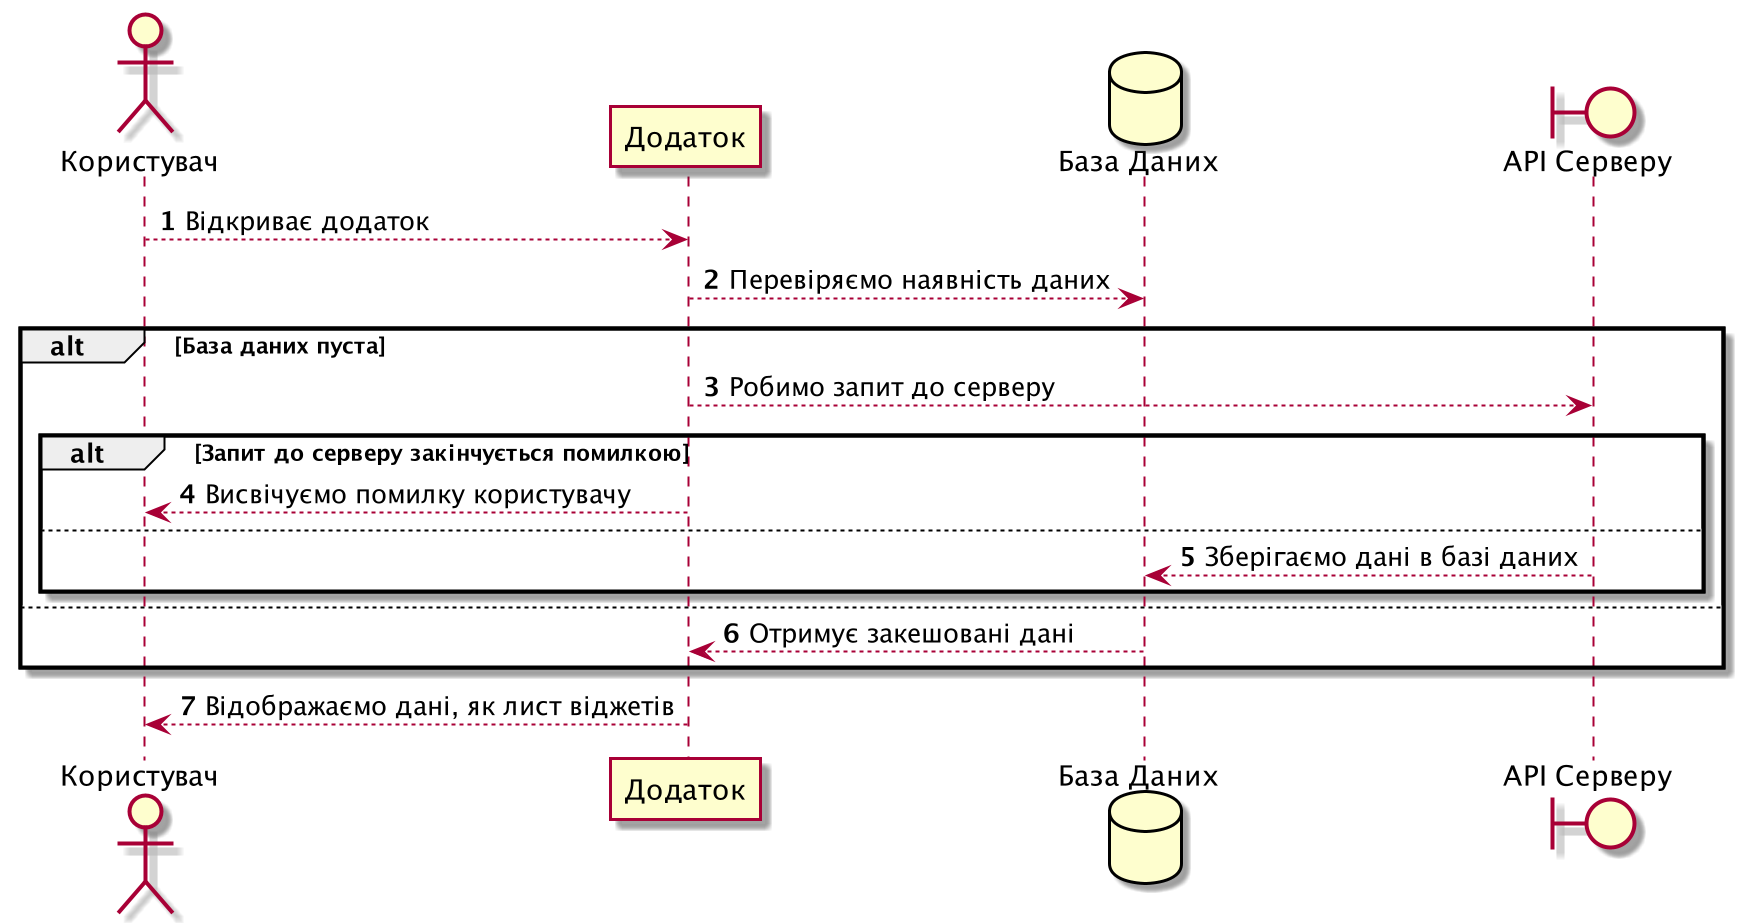
\includegraphics[scale=0.25]{general_app_flow.png}
        \caption{Загальна схема послідовностей додатку}
        \label{fig:gen_app_flow}
    \end{center}
\end{figure}

В якості архітектурного рішення всі додатки імітують архітектуру MVVM(Model-View-View Model) (див. мал. \ref{fig:gen_app_architecture}).
\textbf{ViewModel} - це контроллер, що відповідає за комунікацію з Model рівнем та повертає структуру даних адаптовану під рівень презентації.
\textbf{Model} - це рівень, котрий описує формат рівню даних. На Model рівню ми описуємо контракт взаємодії з даними, як з
мережею так і з базою даних.
\textbf{View} - відповідає за відображення даних, по суті будучи пасивним спостерігачем даних з рівня ViewModel.

\begin{figure}
    \begin{center}
        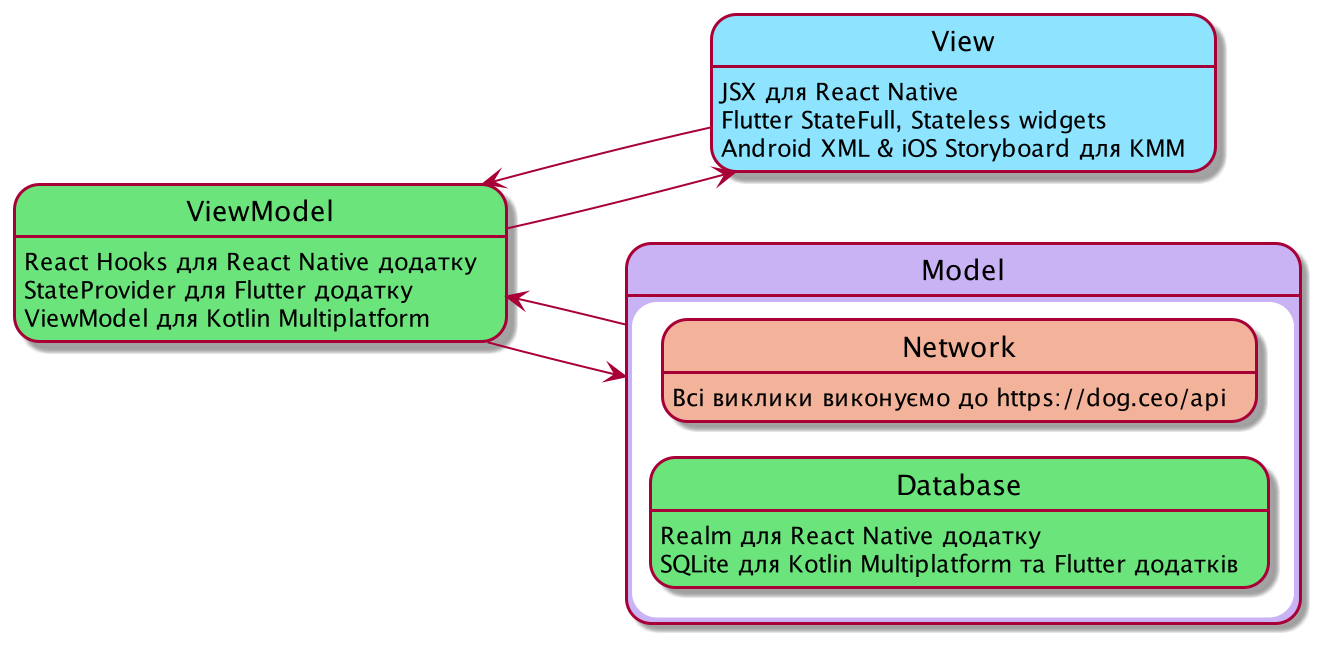
\includegraphics[scale=0.3]{app_layers.png}
        \caption{Загальна архітектура додатку}
        \label{fig:gen_app_architecture}
    \end{center}
\end{figure}

\section{Архітектура додатку React Native}
\label{sec:kn_app_architecture}
В реалізації додатку React Native ми використали систему звротніх викликів або так званих "хуків".
Наприклад, \textbf{useState} - це Хук, що дозволяє додавати стан React до функціональних компонентів.

"useState" оголошує "змінну стану" та повертає пару значень: поточний стан та функцію, яка його оновлює.
Наша змінна називається, data ми можемо називати її як завгодно, наприклад banana \ref{lst:rn_state_hooks}.

Використовуючи useEffect хук, ми повідомляємо React, що наш компонент повинен виконати додаткову фунцію після рендерингу.
React запам'ятає передану нами функцію (яку ми будемо називати "ефектом") і викличе її пізніше після оновлення UI нашого додатку.

Ефект котрий ми створили буде виконаний при ініціалізації додатку. І як результат виконання ми отримаємо дані з локальної бази які ми і відобразимо (див. на \ref{fig:rn_realm})).

\begin{figure}
    \begin{center}
        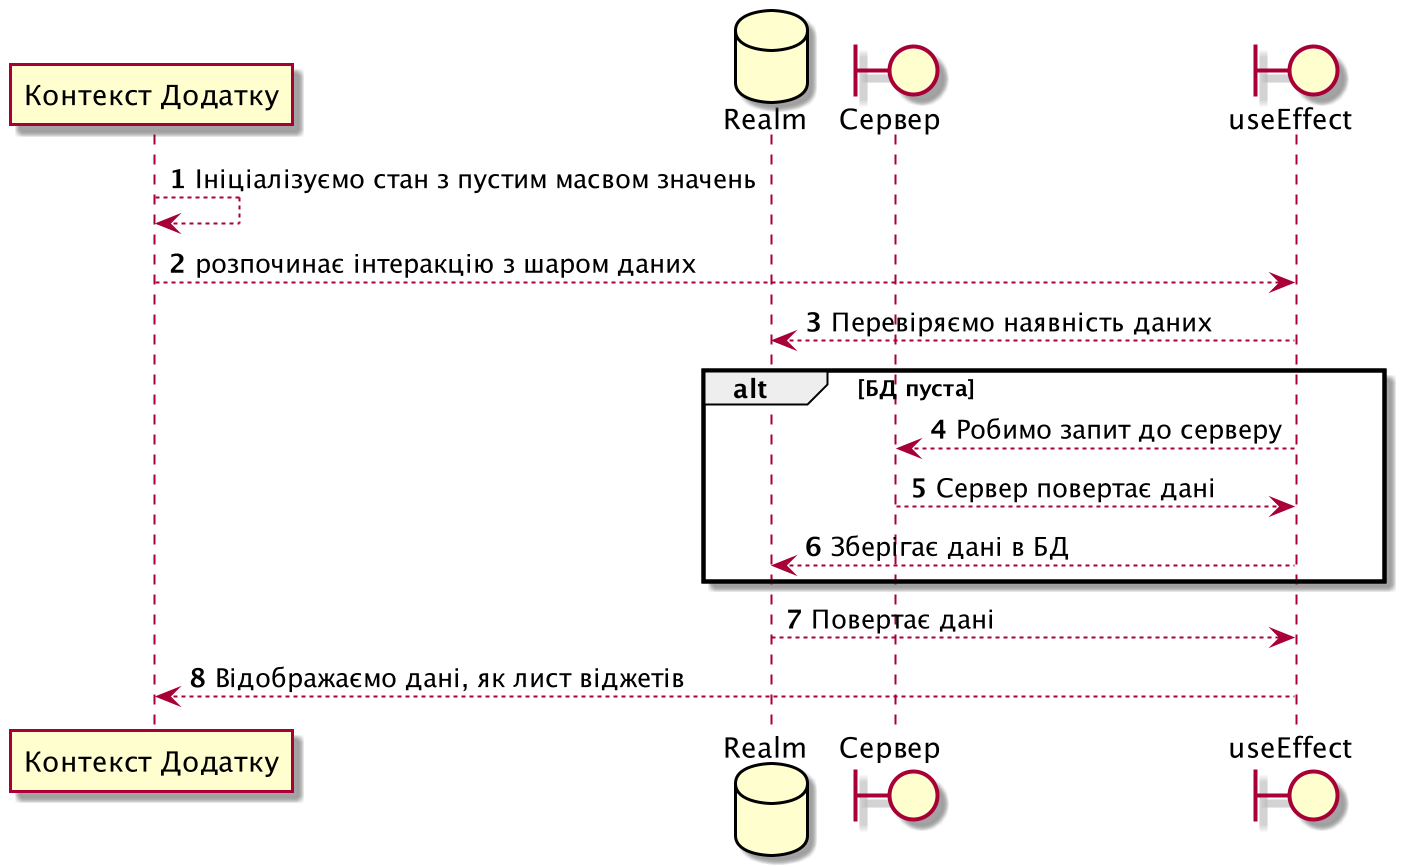
\includegraphics[scale=0.3]{app_widget.png}
        \caption{Схема послідовності віджету App та інтеракція з шаром даних}
        \label{fig:rn_realm}
    \end{center}
\end{figure}


\section{Комунікація з мережею в Flutter додатку з http.dart та async/await}
\label{sec:flutter_network_app}
В нашому додатку запит до інтернету описан в наступному описі сирцевого коду \ref{lst:flutter_networking}.

Найголовнішим принципом, котрим ми опируємо в прикладі запиту до інтернету, це використання "обіцянок" на базі dart:async Future<T>.
Асинхронні операції дозволяють нашій програмі завершити роботу, чекаючи закінчення іншої операції.
Результат використання Future API або закінчиться в завершенному стані або незавершенному.

Коли ми вперше виконуємо асинхрону функцію, то отримаємо посилання на незавершену дію, з якої ми очікуємо результат або помилку.
Щоб уникнути розповсюдження помилки до верхнів шарів ми маємо використати try/catch синтаксис.

Як видно з нашого прикладу використання пакету http.dart в по'єднанні з dart:async дає зручне
та швидке розв'язання проблеми створення та прослухання результатів з інтернету.


\section{Комунікація з SQLite БД в Flutter додатку з SQFlite}
\label{sec:flutter_sqflite_app}
Для комунікації з БД в додатку була використана бібліотека SQFlite.
Рішення, що використовує цю бібліотеку можна знайти за наступним посиланнєм \ref{lst:flutter_sqflite}.

Для того щоб, уникнути витік залежності рішення SQFlite було огорнуто в додатковий тип \textbf{BreedDatabase}.
\textbf{BreedDatabase} дає можливість виконання стандартних процедур підключення до БД з розширенням .sqlite
на стандартному шляху до файлу абстрагованого за допомогою \textbf{getDatabasesPath()} API.

Оскільки наша огортка, це вікно в SQL світ, то наш додаток здатен виконувати всі доступні із стандартного набору
SQL операції.


\section{Управління станом в Flutter додатку з Providers API}
\label{sec:flutter_state_app}
Flutter пропонує кілька способів для управління станом. Серед них BLoC, Provider, Statefull Widgets, InheritedWidgets.
В даній роботі ми розглянемо Provider API, котрий взяв за основу систему InheritedWidgets(віджет, що наслідує).
Для того щоби зрозуміти контроль стану з Provider API ми повинні розлянути:

\begin{itemize}
    \item ChangeNotifier - це простий клас, включений до Flutter SDK, який забезпечує повідомлення про зміни своїх слухачів. Іншими словами, якщо щось є ChangeNotifier, ви можете підписатися на його зміни.
    \item ChangeNotifierProvider - це віджет, який надає екземпляр ChangeNotifier своїм нащадкам. Це походить від пакету провайдера.
    \item Consumer - це віджет, що дозволяє нам огорнути будь-який інший віджит далі в ієрархії та зчитати стан з класу, що наслідує ChangeNotifier.
\end{itemize}

В нашому додатку ми використали StateNotifier, котрий обновлює всіх підписників стану.
Так наприклад зміна значення з стану "завантажується" на стан "завантажений" приводить до перебудови віджету \ref{lst:flutter_sqflite}.


\section{Юніт тестування в Flutter додатку}
\label{sec:flutter_unit_testing_app}
Як було вже зазначено, найкращий спосіб контролю якості в проекті це написання та сопроводження коду написанням юнит тестів.
Цей підхід до розробки програмного забезпечення не оминув і розробку під Flutter.

В даній секції ми наведемо приклад тесту написаного для коду бізнес логіки \ref{lst:flutter_unit_test}.
Ми застосуємо пакети test та mockito.
Пакет тест надає доступ до функцій, які дозволяють нам групувати тести.
Пакет mockito надає функціонал, що дозволяє конфігурувати поведінку об'єктів типу mock(заглушка).

Ми маємо дві "рухомі" залежності: шар комунікації з мережею та БД.
Рухомі частини - це те що ми, як користувачі бібліотек http.dart та SQFlite не контролюємо.
Отже, щоб спростити конфігурацію юніт тестування ми замінили реальні об'єкти на об'єкти заглушки.


\section{Комунікація з мережею в KMM додатку з ktor та couroutines}
\label{sec:kmm_ktor}
На даний момент серед кроссплатформених бібліотек, що дозволяє нам моделювання інтернет викликів,
найпоширенішою - є розв'язання Ktor \cite{ktor_home_page}.
В додатку коду, що йде нижче \ref{kmm_ktor} ми розглянемо приклад реалізації клієнта,
що надалі створює з'єднання з API сервісом, що повертає нам список порід собак.

Визначаємо інтерфейс, що повертає нам результат виконання виклику до API \ref{lst:kmm_ktor}.

Важливим момент є те, що функція визначена ключовим словом \textbf{suspend}.
\textbf{suspend} маркерує нашу функцію, як ту, що буде виконувати "блокуючу" операцію.
Виконання викликів до інтернету операція дорога і можевиконуватися секундами.
Створюємо об'єкт Ktor клієнта та конфігуруємо Json Serializer/Deserializer.
\textbf{ensureNeverFrozen} гарантує, що freezing(заморожування) закінчиться помилкою FreezingException.
Дозволяє уникнути небажаного ефекту freezing, що є основою безпечного контролю посилань між паралельними потоками
під час виконання програмою асинхроних викликів.
Реалізуємо функцію інтерфейсу декларуючи посилання, що нам поверне результат.

Як ми бачимо реалізація виклику за допомогою Ktor та Kotlin, хоча виглядає громоздко, але не є складною.
Більшість логіки, що створює сокет і опрацьовуі потік байтів схована за публічним інтерфейсом.
Від клієнта потребується декларування викликів та дизайн DTO(Data Transfer Object - Транспортний Об'єкт Даних),
в нащому випадку це клас, що описує структуру Json відповіді BreedResult.


\section{Комунікація з мережею в KMM додатку з SQLDelight}
\label{sec:kmm_sqldelight}
Для роботи з БД в нашому KMM(Kotlin) проекті було використана SQLDelight \cite{sqldelight_home}.
SQLDelight використовує ідею генерації коду для клієнту на основі SQL визначень описаних в окремому файлі.

Як видно в прикладі з додатку \ref{table_sq_gen} спочатку ми описуємо структуру таблиць за допомогою SQL.
Далі ми надаємо інструкцію \textbf{selectAll}, що буде використана SQLDelight для генерації коду \ref{lst:table_sq_gen}.

Результатом виконання SQL запиту буде посилання на об'єкт типу курсор, що дозволяє в динамічний спосіб зчитати
результат та адуптувати результат до конкретного типу. Таким чином, ми уникаємо написання низькорівневого коду,
в якому дуже просто припуститися помилки. В випадку більш складних схем БД перевага згенерованого коду дозволяє
нам уникати надмірного повторення в написанні коду прослойки для коммунікації з БД.


\section{Юніт тестування в KMM додатку}
\label{sec:kmm_unit_testing}

Як і в випадку інших платформ розробки тестування коду є критичною для розвитку продукту.
KMM і тут не відстає і пропонує розв'язання для тестування.
Оскільк Kotlin підтримує JVM(Java Virtual Machine) середовище ми можемо запускати тести на стороні Linux, Windows та MacOS платформ.

Тести, що супроводжують загальну логіку тримають в відокремленому репозиторії commonTest.
Для конфігурації специфічного для платформи коду виділяють iosTest для iOS та androidTest для Android платформ.

В нашому додатку був написаний простий інтеграційний тест (див. \ref{lst:kotin_test_common}).
Дуже важливо підкреслити наявність ф-цій \textbf{testDbConnection} та \textbf{runTest}.
Де \textbf{testDbConnection} абстрагує реалізацію драйверу підключення до БД та буде реалізована для кожної
з платформ в своєму специфічному вихідному наборі (ios, android).
\textbf{runTest} абстрагує реалізацію логіку запуску тесту.
Модель багатопотоковість унікальна для кожної з платформ, тому впроваджується абстракція та конкретна імплементація
для кожної з платформ.

Важливо зауважити, що ми базуємо наше рішення на базі специфічної для KMM пари \textbf{expect} та \textbf{actual}.
Дані ключові слова маркерують ф-ції, як ті що залежать від API специфічного для платформи.

В \ref{lst:kotin_test_ios} ми використовуємо в якості реалізації драйвер специфічний для iOS платформи.

В \ref{lst:kotin_test_android} ми використовуємо в якості реалізації драйвер специфічний для Android платформи.

З наведених приклавдів можно зробити висновок, що KMM намагається максимально тісно співпрацювати з API специфічний для платформи.
Таке рішення потребує знання не тільки специфіки Kotlin але й розуміння бібліотек специфічних для платформ.
Тобто KMM не будує додатковий рівень абстракції, що ховає доступ до конкретних специфікацій.
